\chapter{Adaptation d'un maillage de surface dynamique}


\textit{Objectif du chapitre: on veut mettre au point une méthodologie pour déformer un maillage de l'interface en propagation en utilisant le modèle \brep\ dynamique comme support géométrique, afin de pouvoir réaliser des simulations EF/VF dans des domaines de géométrie déformable.}
%\par
%(Motivation : les méthodes (EF, VF, \ldots) employées pour la simulation numérique nécessitent un \textit{maillage} du (volume du) domaine de calcul)


%\section{Problématiques et état de l'art}

%\subsection{Simulation numérique dans un domaine à géométrie déformable}
%Motivation :
%\begin{enumerate}
%	\item les méthodes (EF, VF, \ldots) employées pour la simulation numérique nécessitent un \textit{maillage} du (volume du) domaine de calcul
%	%\item la précision et la vitesse de convergence du calcul dépendent fortement de la qualité (forme et taille) des éléments du maillage
%\end{enumerate}
\section{Simulation numérique dans un domaine à géométrie déformable}
État de l'art :
\begin{enumerate}
	\item maillage volumique (fluide) conforme à l'interface
	\begin{enumerate}
		\item \label{item:methodo_bodyfitted_ALE} un seul maillage \anglais{body-fitted} avec formulation ALE \emph{(ref)}
		\begin{itemize}
			\item principe : frontière = maillage de l'interface, intérieur déformé de façon arbitraire (purement lagrangien si la vitesse de déformation du maillage est imposée par le champ de vitesse du fluide)
			\item intérêt/avantages : \ldots
			\item contraintes/inconvénients : 
			\begin{itemize}
				\item la qualité du maillage volumique dépend fortement de celle du maillage surfacique, surtout dans les régions proches de l'interface, où ont généralement lieu les phénomènes physiques les plus pertinents
				\item la connectivité du maillage doit rester fixe \emph{(à vérifier)}
			\end{itemize}
		\end{itemize}
		
		\item plusieurs maillages \anglais{body-fitted} qui se superposent
		\begin{itemize}
			\item méthode Chimère \cite{meakin1989, wang2000}, FLUSEPA \cite{brenner1991}
			\item intérêt/avantages : 
			\begin{itemize}
				\item facilite la génération du maillage volumique lorsque la géométrie est complexe (\eg hyper-sustentateurs)
				\item évite de déformer un maillage \troisD
			\end{itemize}						
			\item contraintes/inconvénients : 
			\begin{itemize}
				\item nécessite de traiter les intersections entre les blocs de maillage
				\item limité aux mouvements rigides \emph{(à vérifier)}
			\end{itemize}
		\end{itemize}
	\end{enumerate}
	
	\item maillage volumique non-conforme à l’interface
	\begin{itemize}
		\item méthode des frontières immergées \cite{peskin2002, hovnanian2012, wang2012} : interface représentée explicitement, volume (fluide) traité de façon eulérienne (\ie maillage fixe)
		\item intérêt/avantages : évite de générer et déformer un maillage \troisD\ autour d’une géométrie complexe
		\item contraintes/inconvénients : application indirecte des conditions aux limites
	\end{itemize}
\end{enumerate}


\section{Problématiques}
Dans cette thèse,
\begin{enumerate}
	\item on ne traite que le maillage (surfacique) de l'interface
	\item on se concentre sur des maillages triangulaires linéaires par morceaux, mais une extension aux maillages hybrides et courbes est envisageable
	%
	\item on dispose d'un \textit{modèle \brep}
	\begin{enumerate}[label=(\arabic*)]
	    \item décrivant une surface $\interfacebrep$ qui est une bonne approximation de la véritable interface $\interface$ ; \label{item:brep_fidele_interface}
	    \item dynamique, \ie disponible à chaque instant de la propagation ; \label{item:brep_dynamique}
	    \item dont la topologie (\ie le nombre de face, arêtes et sommets et/ou leurs relations d'adjacence) peut évoluer au cours du temps. \label{item:brep_topologie_variable}
	\end{enumerate}
	%
	\item on veut maintenant un \textit{maillage surfacique}
	\begin{enumerate}[label=(\alph*)]
	    \item géométriquement fidèle à l'interface $\interface$ ; \label{item:maillage_fidele_interface}
	    \item dynamique ; \label{item:maillage_dynamique}
	    \item valide et de bonne qualité tout au long de la propagation, afin d'assurer le bon déroulement du calcul (vitesse de convergence et précision) ; \label{item:maillage_qualite}
	    \item dont la connectivité varie le moins possible au cours du temps, afin de ne pas avoir à interpoler/projeter la solution sur un nouveau maillage (généralement coûteux, non-conservatif, introduit de la diffusion numérique \ldots) \label{item:maillage_connectivite_fixe}
	\end{enumerate}
	%
	\item En raison de \ref{item:brep_fidele_interface}, on change le critère \ref{item:maillage_fidele_interface} en : ``géométriquement fidèle à la surface $\interfacebrep$ décrite par le modèle \brep'' \label{item:maillage_fidele_surface_brep}
	\begin{itemize}[label=$\rightarrow$]
        \item le maillage interpole $\interfacebrep$ aux n\oe uds : chaque n\oe ud est repéré sur une (ou plusieurs) entité(s) \brep\ par des coordonnées \textit{paramétriques}
        
        \item on contrôle/limite l'écart de corde en
        \begin{itemize}
            \item spécifiant une carte de taille adaptée à la courbure locale dans les régions régulières\footnote{attention, la continuité $\contgeom{1}$ autorise des discontinuité de courbure, on doit donc assurer la gradation de la carte.}
            \item \label{item:discretisation_singularites} maillant explicitement les singularités géométriques (pics et crêtes)
        \end{itemize}
    \end{itemize}
    
    \item Dans cette thèse, on ne s'intéresse pas tant à la génération du maillage initial %(de nombreuses méthodes qui portent sur ce sujet ont déjà fait leurs preuves, y compris dans un contexte de maillage trans-carreaux) 
    qu'à son évolution au cours du temps. 
	Toutefois, dresser un bref état de l'art des méthodes de génération de maillage surfacique basé sur un modèle \brep\ nous permet de cerner les principales problématiques rencontrées lorsqu'on fait évoluer un tel maillage.
\end{enumerate}


\subsection{Génération de maillage surfacique basé sur un modèle \brep}
%Essentiellement extension de méthodes standard (\ie quadtree, Delaunay, avancée de front) \deuxD\ plan à des surfaces immergées/plongées dans $\reals^3$
\begin{enumerate}
	\item méthodes indirectes (Riemanniennes) : on travaille dans l'espace paramétrique en tenant compte de la métrique (anisotrope, Riemannienne) induite par la paramétrisation de façon à ce que le plongement du maillage dans $\reals^3$ respecte les critères prescrits
	\begin{enumerate}
		\item \textit{carreau-par-carreau} (\ie conforme à la topologie du modèle \brep) : on exploite directement les paramétrisations locales (carreaux de surface) du modèle \brep\ \cite{borouchaki2000} (on maille d'abord les sommets, puis les arêtes et enfin les faces afin de garantir la conformité du maillage)
		\begin{itemize}
			\item intérêt/avantages : utilisation de méthodes \deuxD\ plan robustes et efficaces
			\item contraintes/inconvénients : les arêtes \brep\ régulières introduisent des contraintes supplémentaires sur le maillage, sans avoir de signification du point du vue du calcul EF/VF $\Rightarrow$ éléments de mauvaise qualité
		\end{itemize}
		\item \textit{trans-carreaux} par (re-)paramétrisation globale : l'idée générale est de construire une transformation affine par morceaux (par triangles) l'espace $uv$ de chaque face et un espace $uv$ global, sans affecter la définition géométrique du modèle \brep\ sous-jacent
			\begin{enumerate}
			
				\item \cite{marcum1999} :
				\begin{enumerate}
					\item on construit d'abord un maillage de référence conforme à la topologie \brep\ d'un ensemble de faces regroupées
					\item \label{item:bouche_trous} on bouche artificiellement les éventuels \guillemets{trous} afin qu'il n'y ait qu'un seul bord
					\item on plonge ce maillage dans un espace paramétrique global :
					\begin{itemize}
						\item afin d'obtenir les coordonnées paramétriques globales des n\oe uds intérieurs, on résout un système d'équations elliptique (opérateur Laplacien combinatoire) avec une condition de Dirichlet pour fixer les n\oe uds du bord sur un cercle
						\item on modifie les coordonnées paramétriques globales des n\oe uds du bord afin d'améliorer la forme des éléments incidents
						\item (on répète le processus jusqu'à ce que la qualité des éléments dans l'espace paramétrique global soit convenable)
					\end{itemize}
					\item on élimine les éventuels éléments fictifs créés à l'étape \ref{item:bouche_trous}
					\item on génère une triangulation dans l'espace paramétrique global par avancée de front en utilisant le maillage de référence comme approximation géométrique dans l'espace physique
					\item on retrouve les coordonnées paramétriques locales des n\oe uds du nouveau maillage 
					\item limites : le groupe de faces doit avoir au moins un bord
				\end{enumerate}
				
				\item \cite{noel2002} : 
				\begin{enumerate}
					\item le domaine paramétrique de chaque face \brep\ est décomposé en cellules triangulaires s'appuyant sur les contours
					\item chaque cellule (courbe) est en bijection avec un triangle (linéaire) dans l'espace paramétrique global de la nappe
					\item une triangulation du domaine paramétrique global (convexe) est générée (quadtree-Delaunay) 
					\item limites : le groupe de faces doit avoir au moins un bord
				\end{enumerate}
				
				\item \cite{jones2004} :
				\begin{enumerate}
					\item on part ici aussi d'une triangulation de référence conforme à la topologie \brep\ (\ie chaque face a sa propre triangulation)
					\item l'assemblage des faces en nappes est réalisé directement dans le plan $(u,v)$ à partir des plongements de leur triangulation respective dans leur espace paramétrique local
					\item une face de ``base'' est choisie, le plongement de sa triangulation dans l'espace paramétrique global est identique à celui dans son espace paramétrique local
					\item les triangulations des faces adjacentes sont ensuite plongées une à une dans l'espace $uv$ global à l'aide d'une technique d'avancée de front qui préserve la forme des triangles
					\item limites : 
					\begin{itemize}
						\item cette approche peut échouer si les plongements des triangulations de deux faces adjacentes dans leur espace $uv$ respectif ont des rapports d'échelles différents au niveau d'une arête commune %suivant les deux directions paramétriques
						\item il semblerait que les groupes de faces doivent ici aussi avoir au moins un bord
					\end{itemize}
					
				\end{enumerate}
			\end{enumerate}
		\begin{itemize}
			\item intérêt/avantages : lève les contraintes topologiques du modèle \brep\ qui ne sont pas pertinentes pour le calcul EF/VF, sans en affecter la définition géométrique
			\item limites/inconvénients : 
			\begin{itemize}
				\item topologie : limité aux groupes de faces avec un ou plusieurs bords $\Rightarrow$ nécessite un découpage (généralement manuel) de l'interface
				\item géométrie : limité aux groupes de faces quasi-plans
			\end{itemize}
			
		\end{itemize}
	\end{enumerate}
	
	\item méthodes directes : 
	\begin{enumerate}
		\item \cite{lau1996} : avancée de front directement dans $\reals^3$ avec projection sur la surface exacte des n\oe uds au cours de la génération $\to$ limité à une paramétrisation continue (\ie carreau-par-carreau)
		\item \cite{foucault2013} : avancée de front directe trans-carreaux
	\end{enumerate}
\end{enumerate}

Bilan : conformer le maillage à la topologie du modèle \brep\ introduit de nombreuses contraintes \textit{topologiques} qui ne sont pas pertinentes du point de vue du calcul\footnote{d'où le ``géométriquement'' dans le critère \ref{item:maillage_fidele_surface_brep}.}. 
Ces contraintes nuisent au respect des deux critères \ref{item:maillage_qualite} et \ref{item:maillage_connectivite_fixe}. 
En effet, 
\begin{itemize}
	\item certaines faces \brep\ peuvent comporter des régions (délimitées par des arêtes régulières) plus étroites que la taille de maille prescrite ;
	\item la topologie \brep\ pouvant varier au cours du temps (\cf \ref{item:brep_topologie_variable}), il n'est généralement pas possible de maintenir la conformité maillage-\brep\ sans modifier la connectivité du maillage (même si la topologie (\ie le genre) de l'interface ne change pas, \eg lorsque des arêtes vives convexes ou des sommets vifs non-concaves engendrent des nouveaux carreaux et donc des nouvelles faces, arêtes et sommets réguliers, comme vu dans la \autoref{section:construction_EdS_partielle}).
\end{itemize}



\subsection{Évolution d'un maillage sur un modèle \brep\ dynamique}
\label{section:evolution_maillage_carreau-par-carreau_sur_brep_dynamique}

Un problème inhérent aux méthodes lagrangiennes de suivi d'interface est la formation d'éléments de maillage dégénérés dans les régions concaves de forte courbure. 
Ceci est d'autant plus vrai dans le cas d'une interface régulière par morceaux qui ont une courbure infinie aux points irréguliers (crêtes et pics). Ces méthodes doivent en effet mettre en \oe uvre un traitement spécifique afin d'éviter la formation d'éléments de maillage dégénérés (limitation du pas de temps, mouvement tangentiel, \ldots) \textit{(citer références et illustrer)}.\par 
L'approche décrite dans cette thèse --- qui repose sur l'utilisation d'un modèle \brep\ dynamique composé de carreaux restreints --- permet de résoudre les auto-intersections de l'interface dans ces régions (en délimitant les régions actives des carreaux). 
Cependant, lorsqu'un maillage est \guillemets{collé} sur le modèle \brep\ dynamique, le problème de la validité des éléments de maillage proche des arêtes vives concaves se pose à nouveau.
\par
%La méthode proposée au paragraphe précédent ne permet ainsi pas d'assurer la validité du maillage déformé.
%On peut décomposer cette évolution en peut être décomposée en 
%    \begin{itemize}
%        \item une évolution géométrique (\ie déformation) :
%        \begin{itemize}
%            \item mouvement de \textit{propagation} imposé par la surface \brep\ dynamique ; \label{item:deformation_propagation}
%            \item mouvement de \textit{glissement} (\ie tangentiel) sur la surface \brep\ (phase d'optimisation par bouger de n\oe ud) ; \label{item:deformation_glissement}
%        \end{itemize}
%        \item une évolution topologique : modifications locales de la connectivité (à éviter autant que possible, \cf \ref{item:maillage_connectivite_fixe}).
%    \end{itemize}
%
Considérons dans un premier temps le cas d'un maillage carreau-par-carreau. 
Un moyen simple de faire évoluer un tel maillage au cours du temps consiste à %figer les coordonnées paramétriques des n\oe uds sur les carreaux qui évoluent. 
\begin{enumerate}
	\item mettre à jour la position\footnote{\label{foot:position_uv_xyz}non seulement dans l'espace physique mais également dans les espaces paramétriques des carreaux incidents.} des n\oe uds associés aux sommets \brep\ ;
	\item pour chaque arête \brep, régénérer une discrétisation\footref{foot:position_uv_xyz} optimale qui préserve le nombre de n\oe uds (\eg en revisitant la procédure de tracé des polylignes d'intersection, \cf \autoref{trace_courbes_intersection}) ;
	\item figer les coordonnées paramétriques de tous les autres n\oe uds, dont la position dans l'espace physique évolue alors avec la définition des carreaux sous-jacents.
\end{enumerate}
Ainsi, on impose indirectement au maillage le mouvement de propagation de l'interface. 
%
En suivant cette approche, si le pas de temps choisi est trop grand (\textit{expliciter contrainte sur le pas de temps, \cf figure GeoGebra}) alors 
\begin{itemize}
	\item certains triangles incidents à la singularité peuvent être inversés ;
	\item les n\oe uds responsables de ces inversions résident dans des régions des carreaux qui sont désormais inactives, et ne sont donc plus supportés par des faces \brep.
\end{itemize}

Il est donc nécessaire de resituer ces n\oe uds dans des régions actives, tout en veillant à ce que leurs triangles incidents aient la bonne orientation. 
Afin de remédier à ce problème, on peut par exemple interpoler le mouvement des n\oe uds du contour de chaque face pour placer tous les n\oe uds libres à l'intérieur du nouveau domaine paramétrique de la face (\textit{\cf papier IMR}).
\par
Avant de considérer le cas d'un maillage trans-carreau, on passe brièvement en revue les méthodes utilisées pour améliorer la qualité du maillage. 
En effet, si la validité de ce dernier peut être maintenue de la façon décrite plus haut, sa qualité peut être sévèrement dégradée au cours de la propagation, jusqu'à compromettre le bon déroulement de la simulation numérique.


\subsection{Optimisation de maillage surfacique}
\setlength{\imagewidth}{18mm}%
\setlength{\imageheight}{\imagewidth}%
\def\swapbend{66}
\def\vertexradius{1.5pt}
\begin{figure}
	\centering
	%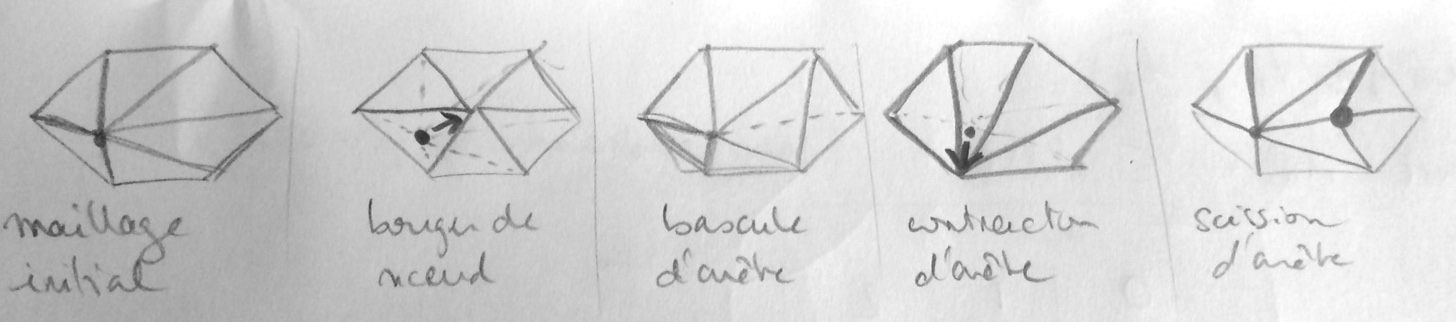
\includegraphics[width=\textwidth]{operations_locales_optimisation_maillage}
	\begin{tikzpicture}[
		x=\imagewidth,
		y=\imageheight,
		mesh/.style={draw=black, semithick},
		label/.style={anchor=south west, inner sep=0},
		optim/.style={mycolor_2, line width=2.0pt},
		arrow/.style={optim , -stealth}, 
		move/.style={arrow, shorten <=2pt, shorten >=3pt},
		swap/.style={arrow, shorten <=1pt, shorten >=1pt},
		%collapse/.style={arrow, shorten <=2pt, shorten >=3pt},
		collapse/.style={optim, dashed},
		before/.style={draw=black!30!white, dashed, thin},
		vertex/.style={fill=black, draw=none, circle, scale=0.3, inner sep=0},
	]
		\begin{scope}[shift={(0.0, -0)}]
	\draw[mesh] 
		(0.08373422920703888, 0.9040214419364929) -- (-0.8304623365402222, 0.49192529916763306)
		(-0.5802370309829712, 0.24899999797344208) -- (0.8759713172912598, -0.40999728441238403)
		(-0.5802370309829712, 0.24899999797344208) -- (0.08373422920703888, 0.9040214419364929)
		(-0.5802370309829712, 0.24899999797344208) -- (0.8661928772926331, 0.48200759291648865)
		(0.8759713172912598, -0.40999728441238403) -- (0.8661928772926331, 0.48200759291648865)
		(-0.5802370309829712, 0.24899999797344208) -- (-0.8304623365402222, 0.49192529916763306)
		(0.0585169717669487, -0.770743727684021) -- (0.8759713172912598, -0.40999728441238403)
		(0.08373422920703888, 0.9040214419364929) -- (0.8661928772926331, 0.48200759291648865)
		(-0.5802370309829712, 0.24899999797344208) -- (-0.7628560066223145, -0.4127168357372284)
		(-0.8304623365402222, 0.49192529916763306) -- (-0.7628560066223145, -0.4127168357372284)
		(-0.5802370309829712, 0.24899999797344208) -- (0.0585169717669487, -0.770743727684021)
		(-0.7628560066223145, -0.4127168357372284) -- (0.0585169717669487, -0.770743727684021)
		;
	\node[label] at (-0.866025403784, -0.83) {(a)};
\end{scope}
\begin{scope}[shift={(1.19802540378, -1.82004086811)}]
	\draw[before] 
		(0.08373422920703888, 0.9040214419364929) -- (-0.8304623365402222, 0.49192529916763306)
		(-0.5802370309829712, 0.24899999797344208) -- (0.8759713172912598, -0.40999728441238403)
		(-0.5802370309829712, 0.24899999797344208) -- (0.08373422920703888, 0.9040214419364929)
		(-0.5802370309829712, 0.24899999797344208) -- (0.8661928772926331, 0.48200759291648865)
		(0.8759713172912598, -0.40999728441238403) -- (0.8661928772926331, 0.48200759291648865)
		(-0.5802370309829712, 0.24899999797344208) -- (-0.8304623365402222, 0.49192529916763306)
		(0.0585169717669487, -0.770743727684021) -- (0.8759713172912598, -0.40999728441238403)
		(0.08373422920703888, 0.9040214419364929) -- (0.8661928772926331, 0.48200759291648865)
		(-0.5802370309829712, 0.24899999797344208) -- (-0.7628560066223145, -0.4127168357372284)
		(-0.8304623365402222, 0.49192529916763306) -- (-0.7628560066223145, -0.4127168357372284)
		(-0.5802370309829712, 0.24899999797344208) -- (0.0585169717669487, -0.770743727684021)
		(-0.7628560066223145, -0.4127168357372284) -- (0.0585169717669487, -0.770743727684021)
		;
	\draw[mesh] 
		(0.08373422920703888, 0.9040214419364929) -- (-0.8304623365402222, 0.49192529916763306)
		(0.0485161654651165, 0.0474160760641098) -- (0.8759713172912598, -0.40999728441238403)
		(0.0485161654651165, 0.0474160760641098) -- (0.08373422920703888, 0.9040214419364929)
		(0.0485161654651165, 0.0474160760641098) -- (0.8661928772926331, 0.48200759291648865)
		(0.8759713172912598, -0.40999728441238403) -- (0.8661928772926331, 0.48200759291648865)
		(0.0485161654651165, 0.0474160760641098) -- (-0.8304623365402222, 0.49192529916763306)
		(0.0585169717669487, -0.770743727684021) -- (0.8759713172912598, -0.40999728441238403)
		(0.08373422920703888, 0.9040214419364929) -- (0.8661928772926331, 0.48200759291648865)
		(0.0485161654651165, 0.0474160760641098) -- (-0.7628560066223145, -0.4127168357372284)
		(-0.8304623365402222, 0.49192529916763306) -- (-0.7628560066223145, -0.4127168357372284)
		(0.0485161654651165, 0.0474160760641098) -- (0.0585169717669487, -0.770743727684021)
		(-0.7628560066223145, -0.4127168357372284) -- (0.0585169717669487, -0.770743727684021)
		;
	\fill[black] (0.0485161654651165,0.0474160760641098) circle (\vertexradius);
	\draw[move] (-0.5802370309829712,0.24899999797344208) -- (0.0485161654651165,0.0474160760641098);
	\node[label] at (-0.866025403784, -0.83) {(b)};
\end{scope}
\begin{scope}[shift={(2.39605080757, -0)}]
	\draw[before] 
		(0.08373422920703888, 0.9040214419364929) -- (-0.8304623365402222, 0.49192529916763306)
		(-0.5802370309829712, 0.24899999797344208) -- (0.8759713172912598, -0.40999728441238403)
		(-0.5802370309829712, 0.24899999797344208) -- (0.08373422920703888, 0.9040214419364929)
		(-0.5802370309829712, 0.24899999797344208) -- (0.8661928772926331, 0.48200759291648865)
		(0.8759713172912598, -0.40999728441238403) -- (0.8661928772926331, 0.48200759291648865)
		(-0.5802370309829712, 0.24899999797344208) -- (-0.8304623365402222, 0.49192529916763306)
		(0.0585169717669487, -0.770743727684021) -- (0.8759713172912598, -0.40999728441238403)
		(0.08373422920703888, 0.9040214419364929) -- (0.8661928772926331, 0.48200759291648865)
		(-0.5802370309829712, 0.24899999797344208) -- (-0.7628560066223145, -0.4127168357372284)
		(-0.8304623365402222, 0.49192529916763306) -- (-0.7628560066223145, -0.4127168357372284)
		(-0.5802370309829712, 0.24899999797344208) -- (0.0585169717669487, -0.770743727684021)
		(-0.7628560066223145, -0.4127168357372284) -- (0.0585169717669487, -0.770743727684021)
		;
	\draw[mesh] 
		(0.08373422920703888, 0.9040214419364929) -- (-0.8304623365402222, 0.49192529916763306)
		(-0.5802370309829712, 0.24899999797344208) -- (0.8759713172912598, -0.40999728441238403)
		(-0.5802370309829712, 0.24899999797344208) -- (0.08373422920703888, 0.9040214419364929)
		(-0.5802370309829712, 0.24899999797344208) -- (0.8661928772926331, 0.48200759291648865)
		(0.8759713172912598, -0.40999728441238403) -- (0.8661928772926331, 0.48200759291648865)
		(-0.5802370309829712, 0.24899999797344208) -- (-0.8304623365402222, 0.49192529916763306)
		(0.0585169717669487, -0.770743727684021) -- (0.8759713172912598, -0.40999728441238403)
		(0.08373422920703888, 0.9040214419364929) -- (0.8661928772926331, 0.48200759291648865)
		(-0.5802370309829712, 0.24899999797344208) -- (-0.7628560066223145, -0.4127168357372284)
		(-0.8304623365402222, 0.49192529916763306) -- (-0.7628560066223145, -0.4127168357372284)
		(-0.7628560066223145, -0.4127168357372284) -- (0.0585169717669487, -0.770743727684021)
		(0.8759713172912598, -0.40999728441238403) -- (-0.7628560066223145, -0.4127168357372284)
		;
	\draw[swap] (-0.26086002588272095,-0.26087185740470886) to [bend left=\swapbend] (0.056557655334472656,-0.411357045173645);
	\node[label] at (-0.866025403784, -0.83) {(c)};
\end{scope}
\begin{scope}[shift={(3.59407621135, -1.82004086811)}]
	\draw[before] 
		(0.08373422920703888, 0.9040214419364929) -- (-0.8304623365402222, 0.49192529916763306)
		(-0.5802370309829712, 0.24899999797344208) -- (0.8759713172912598, -0.40999728441238403)
		(-0.5802370309829712, 0.24899999797344208) -- (0.08373422920703888, 0.9040214419364929)
		(-0.5802370309829712, 0.24899999797344208) -- (0.8661928772926331, 0.48200759291648865)
		(0.8759713172912598, -0.40999728441238403) -- (0.8661928772926331, 0.48200759291648865)
		(-0.5802370309829712, 0.24899999797344208) -- (-0.8304623365402222, 0.49192529916763306)
		(0.0585169717669487, -0.770743727684021) -- (0.8759713172912598, -0.40999728441238403)
		(0.08373422920703888, 0.9040214419364929) -- (0.8661928772926331, 0.48200759291648865)
		(-0.5802370309829712, 0.24899999797344208) -- (-0.7628560066223145, -0.4127168357372284)
		(-0.8304623365402222, 0.49192529916763306) -- (-0.7628560066223145, -0.4127168357372284)
		(-0.5802370309829712, 0.24899999797344208) -- (0.0585169717669487, -0.770743727684021)
		(-0.7628560066223145, -0.4127168357372284) -- (0.0585169717669487, -0.770743727684021)
		;
	\draw[mesh] 
		(-0.8304623365402222, 0.49192529916763306) -- (0.8759713172912598, -0.40999728441238403)
		(-0.8304623365402222, 0.49192529916763306) -- (0.08373422920703888, 0.9040214419364929)
		(-0.8304623365402222, 0.49192529916763306) -- (0.8661928772926331, 0.48200759291648865)
		(0.8759713172912598, -0.40999728441238403) -- (0.8661928772926331, 0.48200759291648865)
		(0.0585169717669487, -0.770743727684021) -- (0.8759713172912598, -0.40999728441238403)
		(0.08373422920703888, 0.9040214419364929) -- (0.8661928772926331, 0.48200759291648865)
		(-0.8304623365402222, 0.49192529916763306) -- (-0.7628560066223145, -0.4127168357372284)
		(-0.8304623365402222, 0.49192529916763306) -- (0.0585169717669487, -0.770743727684021)
		(-0.7628560066223145, -0.4127168357372284) -- (0.0585169717669487, -0.770743727684021)
		;
	\draw[collapse] (-0.5802370309829712,0.24899999797344208) -- (-0.8304623365402222,0.49192529916763306);
	\node[label] at (-0.866025403784, -0.83) {(d)};
\end{scope}
\begin{scope}[shift={(4.79210161514, -0)}]
	\draw[mesh] 
		(0.08373422920703888, 0.9040214419364929) -- (-0.8304623365402222, 0.49192529916763306)
		(0.1478671431541443, -0.08049865067005157) -- (0.8759713172912598, -0.40999728441238403)
		(-0.5802370309829712, 0.24899999797344208) -- (0.08373422920703888, 0.9040214419364929)
		(-0.5802370309829712, 0.24899999797344208) -- (0.8661928772926331, 0.48200759291648865)
		(0.8759713172912598, -0.40999728441238403) -- (0.8661928772926331, 0.48200759291648865)
		(-0.5802370309829712, 0.24899999797344208) -- (-0.8304623365402222, 0.49192529916763306)
		(0.0585169717669487, -0.770743727684021) -- (0.8759713172912598, -0.40999728441238403)
		(0.08373422920703888, 0.9040214419364929) -- (0.8661928772926331, 0.48200759291648865)
		(-0.5802370309829712, 0.24899999797344208) -- (-0.7628560066223145, -0.4127168357372284)
		(-0.8304623365402222, 0.49192529916763306) -- (-0.7628560066223145, -0.4127168357372284)
		(-0.5802370309829712, 0.24899999797344208) -- (0.0585169717669487, -0.770743727684021)
		(-0.7628560066223145, -0.4127168357372284) -- (0.0585169717669487, -0.770743727684021)
		(0.1478671431541443, -0.08049865067005157) -- (-0.5802370309829712, 0.24899999797344208)
		(0.1478671431541443, -0.08049865067005157) -- (0.8661928772926331, 0.48200759291648865)
		(0.0585169717669487, -0.770743727684021) -- (0.1478671431541443, -0.08049865067005157)
		;
	\fill[black] (0.1478671431541443,-0.08049865067005157) circle (\vertexradius);
	\node[label] at (-0.866025403784, -0.83) {(e)};
\end{scope}

	\end{tikzpicture}
	\caption{Opérations élémentaires d'optimisation de maillage surfacique. (a) Maillage initial. (b) Bouger de n\oe ud. (c) Bascule d'arête. (d) Contraction d'arête. (e) Scission d'arête (insertion de n\oe ud).}
	\label{fig:operations_locales_optimisation_maillage}
\end{figure}

\subsubsection{Opérateurs élémentaires}
\begin{enumerate}
	\item bouger de n\oe ud (direct, \ie $xyz$ ou indirect, \ie $uv$)
	\begin{enumerate}
		\item méthodes heuristiques : lissage laplacien, analogies physiques \cite{farhat1998}, interpolation (IDW, RBF, \ldots)
		\item lissage basé sur l'optimisation d'une métrique de qualité \cite{freitag1995, canann1998, jiao2008, gargallo2014}
	\end{enumerate}
	\item changements locaux de connectivité
	\begin{enumerate}
		\item bascule d'arête
		\item contraction d'arête
		\item scission d'arête
	\end{enumerate}
\end{enumerate}

\subsubsection{Optimisation de maillage surfacique reposant sur un modèle \brep} 
\begin{enumerate}
	\item bouger de n\oe ud carreau-par-carreau : \cite{gargallo2014}
	\item trans-carreaux : \cite{noel1995}
\end{enumerate}








Bilan : 
Des méthodes de \textit{génération} et d'\textit{adaptation} de maillage \textit{trans-carreaux} à partir de modèles \brep\ \textit{statiques} \cite{noel1995, foucault2008} ainsi que des méthodes de \textit{déformation (adaptation)} de maillage \textit{carreau-par-carreau} à partir de modèles \brep\ \textit{dynamiques} \cite{martin2017} ont déjà fait l'objet de plusieurs travaux. 
(Certains travaux \cite{louhichi2015} ont également considéré l'approche inverse, à savoir la reconstitution d'un modèle \brep\ à partir d'un maillage déformé à l'issue d'un calcul EF. 
Ici aussi, le maillage est conforme aux carreaux et la topologie \brep\ ne change pas, la déformation étant dictée par un champ vectoriel de déplacement continu.)
\par
Dans cette thèse, on propose une méthodologie pour \textit{adapter} un maillage \textit{trans-carreaux} basé sur un modèle \brep\ \textit{dynamique} (ce qui, à ma connaissance, n'a pas encore fait l'objet de travaux publiés).



%\section{Maillage trans-carreaux reposant sur un modèle \brep\ dynamique}
\section{Modèle maximal}
Motivation : on veut que le maillage respecte la \textit{géométrie} du modèle \brep\ (\cf objectif \ref{item:maillage_fidele_surface_brep}), mais pas nécessairement sa \textit{topologie}\\
$\to$ on veut s'affranchir de toutes les contraintes topologiques du modèle \brep\ qui ne sont pas pertinentes du point de vue du calcul EF/VF


%\subsection{Modèle maximal}
Comme nous l'avons vu dans la \autoref{section:description_surface_G1_piecewise}, une surface régulière \piecewise\ peut être décrite comme un ensemble de \textit{nappes}, \textit{crêtes} et \textit{pics}. \par 

\begin{definition}[Modèle maximal]
	On dit qu'une nappe $\nappe_a$ (resp. crête $\crete_a$) est \emph{maximale} s'il n'existe aucune nappe $\nappe_b$ (resp. crête $\crete_b$) telle que $\nappe_a \subset \nappe_b$ (resp. $\crete_a \subset \crete_b$). \par
	On appelle \emph{modèle maximal} d'une surface $\contgeom{1}$ \piecewise\ l'ensemble de ses nappes maximales, crêtes maximales et pics.
\end{definition}

Ainsi, une nappe maximale correspond à un ensemble connexe et globalement $\contgeom{1}$ de faces \brep. 
Une crête maximale correspond à un ensemble connexe et globalement $\contgeom{1}$ d'arêtes \brep\ vives, qui est incident à une ou deux nappe(s) maximale(s) et est délimitée par zéro, un ou deux pic(s).
Enfin, un pic correspond à un sommet \brep\ (vif), et représente l'extrémité d'une ou plusieurs crêtes maximales.\par
%Dans la suite on ne considèrera que des nappes et crêtes maximales.
%On omettra donc le qualificatif \textit{maximal} afin d'alléger le propos.
Essentiellement, la différence entre les modèle \brep\ et maximal est que ce dernier est unique. 
%On ne peut en effet pas assembler deux nappes (resp. crêtes ou pics) pour en former une nouvelle sans en violer la définition donnée dans la \autoref{section:description_surface_G1_piecewise}. 
Regrouper les faces et arêtes d'un modèle \brep\ en nappes et crêtes maximales ne modifie ainsi pas la définition géométrique de la surface qu'il décrit, mais permet d'en fournir une nouvelle représentation, dont la topologie est plus simple. 
Cette représentation, qui était peu pratique pour concevoir un algorithme d'ordre élevé et efficace de propagation d'interface, s'avère maintenant être un outil intéressant pour imposer au maillage un nombre minimal de contraintes topologiques.\par
On décrit dans les paragraphes suivants les procédures permettant de construire explicitement le modèle maximal à partir des entités du modèle \brep.

\subsection{Assemblage des faces \brep\ en nappes maximales}
Pour constituer les nappes maximales, on procède de la manière suivante. 
On commence par marquer toutes les faces du modèle \brep\ comme \textit{non-visitées}. 
Ensuite, pour chaque face non-visitée, on initialise une nouvelle nappe vide que l'on remplit en suivante la procédure récursive décrite par l'\autoref{algo:assembler_nappe}.

\begin{algorithm}
	\caption{Assemblage récursif de faces en une nappe.}\label{algo:assembler_nappe}
	\begin{algorithmic}[1]
		\Procedure{Assembler nappe}{$\brepface$, $\nappe$}
			\State marquer $\brepface$ comme visitée
			\State ajouter $\brepface$ à la nappe $\nappe$
			\For{chaque contour $\brepwire$ de $\brepface$}
				\For{chaque co-arête régulière $\brepedge^i$ de $\brepwire$}
					\If{la face $\brepface_j$ incidente à la co-arête jumelle de $\brepedge^i$ n'a pas déjà été visitée}
						\State \Call{Assembler nappe}{$\brepface_j$, $\nappe$}
					\EndIf
				\EndFor
			\EndFor
		\EndProcedure
	\end{algorithmic}
\end{algorithm}


\subsection{Identification des pics}
Les pics correspondent à des extrémités de crêtes maximales. 
On définit la \textit{valence} d'un sommet \brep\ comme le nombre d'arêtes \brep\ \textit{vives} auxquelles il est incident. 
Sont des pics les sommets
\begin{itemize}
	\item de valence strictement supérieure à 2 ;
	\item de valence égale à 1 (techniquement un tel sommet est un point régulier de l'interface, mais il délimite tout de même une crête) ;
	\item de valence égale à 2, et où les deux arêtes incidentes ont des directions tangentes non-parallèles.
\end{itemize}

Pour le dernier cas, on calcule la direction tangente $\bt_i$ ($i = 1,2$) à chaque arête en exploitant la géométrie différentielle de la courbe d'intersection transverse qui la supporte (voir \autoref{section:representation_intersections}). 
On considère que le sommet commun de ces arêtes est un pic si l'angle entre les directions tangentes dépasse un certain seuil $\epsilon$, \ie si 
\begin{equation}
	\left| \dotprod{\bt_1}{\bt_2} \right| < \cos \epsilon.
\end{equation}



\subsection{Assemblage des arêtes \brep\ vives en crêtes maximales}
Afin d'en simplifier le parcours, on donne une orientation consistante aux crêtes. 
Pour cela, on conçoit une crête comme une suite de \textit{co-arêtes}.
\par
Dans un premier temps, on obtient les crêtes maximales \textit{ouvertes}, \ie qui possèdent deux pics (pas nécessairement distincts\footnote{On traite en effet les crêtes ayant leurs deux extrémités au même pic comme des crêtes ouvertes.}) comme extrémités. 
L'\autoref{algo:former_cretes_ouvertes} qui réalise l'assemblage de ces crêtes consiste à \guillemets{marcher} de pic en pic le long d'arêtes vives en prenant soin de ne parcourir chaque arête qu'au plus une fois. 
Cette procédure de marche est décrite par l'\autoref{algo:assembler_crete}. 
On a obtenu toutes les crêtes ouvertes une fois que toutes les arêtes vives incidentes à chaque pic ont été visitées. 


\begin{algorithm}
	\caption{Obtention des crêtes ouvertes.}\label{algo:former_cretes_ouvertes}
	\begin{algorithmic}[1]
		%\Procedure{Obtenir crêtes ouvertes}{}
			%
			\For{chaque pic $\brepvertex$}
				\For{chaque co-arête vive $\brepedge^i$ non-visitée ayant pour origine $\brepvertex$}
					% comment? parcourir cycle des co-aretes incidentes (twin(prev))
					\State $\crete = $ \Call{Assembler crête}{$\brepedge^i$}
					\State Ajouter $\crete$ à la liste des crêtes
				\EndFor
			\EndFor
		%\EndProcedure
	\end{algorithmic}
\end{algorithm}

\par
On procède alors à l'assemblage des crêtes maximales \textit{fermées}. 
Celles-ci n'ayant pas d'extrémité, on choisit arbitrairement un de leurs sommets intérieurs comme point de départ pour l'assemblage. 
L'\autoref{algo:former_cretes_ouvertes} qui réalise l'assemblage des crêtes fermées utilise également la procédure de marche décrite par l'\autoref{algo:assembler_crete}. 
Cette fois, en revanche, l'assemblage se termine lorsque le sommet destination de la dernière co-arête visitée est identique au sommet de départ. 
On a obtenu toutes les crêtes fermées une fois que chaque arête vive a été visitée exactement une fois. 

\begin{algorithm}
	\caption{Obtention des crêtes fermées.}\label{algo:former_cretes_fermees}
	\begin{algorithmic}[1]
		%\Procedure{Obtenir crêtes fermées}{}
			%
			\For{chaque sommet \brep\ $\brepvertex$ de valence égale à 2 qui n'est pas un pic}
				\State{$\brepedge^i \gets$ co-arête vive ayant pour origine $\brepvertex$}\Comment{celle-ci est unique et n'a pas encore été visitée}
				\State $\crete = $ \Call{Assembler crête}{$\brepedge^i$}
				\State Ajouter $\crete$ à la liste des crêtes
			\EndFor
		%\EndProcedure
	\end{algorithmic}
\end{algorithm}


%
\begin{algorithm}
	\caption{Assemblage de co-arêtes en une crête.}\label{algo:assembler_crete}
	\begin{algorithmic}[1]
		\Procedure{Assembler crête}{$\brepedge_0^i$}
			%
%			\State initialiser une crête $\crete = \left\{ \brepedge_0^i \right\}$
%			\State marquer la co-arête $\brepedge_0^i$ et sa jumelle comme visitées
%			\State{$\brepvertex \gets \dest(\brepedge_0^i)$}
%			\While{$\brepvertex \neq \orig(\brepedge_0^i)$ et $\brepvertex$ n'est pas un pic}
%				%
%				\State{$\brepedge^j \gets$ co-arête vive ayant pour origine $\brepvertex$}\Comment{celle-ci est unique et n'a pas encore été visitée}
%				% comment? parcourir cycle des co-aretes incidentes (twin(prev))
%				\State ajouter $\brepedge^j$ à la crête $\crete$
%				\State marquer la co-arête $\brepedge^j$ et sa jumelle comme visitées
%				\State{$\brepvertex \gets \dest(\brepedge^i)$}
%			\EndWhile
%			\State\Return{$\crete$}
			%
			\State initialiser une crête vide $\crete$
			\State{$\brepedge^j \gets \brepedge_0^i$}
			\While{$\dest(\brepedge^j) \neq \orig(\brepedge_0^i)$ et $\dest(\brepedge^j)$ n'est pas un pic}
				\State ajouter $\brepedge^j$ à la crête $\crete$
				\State marquer la co-arête $\brepedge^j$ et sa jumelle comme visitées
				\State{$\brepedge^j \gets$ co-arête vive ayant pour origine $\dest(\brepedge^j)$}\Comment{celle-ci est unique et n'a pas encore été visitée}
%				\Repeat\Comment{$\brepedge^j \gets$ co-arête vive ayant pour origine $\dest(\brepedge^j)$}
%					\State{$\brepedge^j \gets \prev(\brepedge^j)$}
%					\State{$\brepedge^j \gets \twin(\brepedge^j)$}
%				\Until{$\brepedge^j$ est vive et n'a pas encore été visitée}
			\EndWhile
			\State\Return{$\crete$}
		\EndProcedure
	\end{algorithmic}
\end{algorithm}


\subsection{Liens entre maillage trans-carreaux et modèle maximal}
On choisit donc de conformer le maillage $\maillage$ au modèle maximal de $\interfacebrep$, \ie
    \begin{itemize}
        \item chaque pic de $\interfacebrep$ est représenté par un n\oe ud de $\maillage$ ;
        \item chaque crête maximale de $\interfacebrep$ est représentée par une \textit{chaîne} de n\oe uds de $\maillage$ connectés par une suite d'arêtes ayant la même topologie (\ie mêmes connexité et nombre d'extrémités) ;
        \item chaque nappe maximale de $\interfacebrep$ est représentée par un ensemble de triangles de $\maillage$ ayant la même topologie (\ie mêmes connexité, genre et nombre de bords) ;
        \item puisque le modèle maximal ne fournit aucune nouvelle définition géométrique, chaque n\oe ud est toujours repéré sur des entités \brep\ (contenues dans l'entité maximale à laquelle est associé le n\oe ud) :
        \begin{itemize}
            \item un n\oe ud reposant sur un pic pointe vers le sommet \brep\ qui représente ce pic et, (comme ce dernier) est repéré par ses coordonnées $(u,v)$ dans chacune des faces incidentes ;%\footnote{Objet \texttt{intersection point}} ;
            \item un n\oe ud reposant une crête pointe vers l'arête (contenue dans cette crête) qui le contient, et est donc repéré par ses coordonnées $(u,v)$ dans chacune des deux faces incidentes ;
%            \begin{itemize}
%                \item pointe vers l'arête (contenue dans cette crête) qui le contient, et est donc repéré par ses coordonnées $(u,v)$ dans chacune des deux faces incidentes ;
%                \item (est associé à la chaîne qui le contient (qui est elle-même associée à cette crête)) ;
%            \end{itemize}
            \item un n\oe ud reposant sur une nappe pointe vers la face \brep\ qui le contient, et est repéré par ses coordonnées $(u,v)$ dans cette face.
        \end{itemize}
    \end{itemize}


%\subsection{Cohérence/Persistance du modèle maximal}
%\cf notes ``Virtual topology''


\section{Évolution d'un maillage trans-carreaux reposant sur un modèle \brep\ dynamique}
Les contraintes topologiques imposées sur le maillage sont maintenant minimales (si on veut respecter \ref{item:discretisation_singularites}). 
Afin de satisfaire les exigences \ref{item:maillage_dynamique} et \ref{item:maillage_connectivite_fixe}, il est nécessaire de ré-établir à chaque instant les associations entre les n\oe uds et chaînes du maillage et les entités maximales de l'interface $\interfacebrep$ décrite par le modèle \brep\ dynamique.
%On suppose que ces associations sont établies à l'état initial (\eg en tant que sous-produit du processus de génération de maillage).
%Il suffit alors \ldots

\par\bigskip
\newcommand{\instant}[2]{#1^{(#2)}}
Dans la suite, on note $\instant{A}{i}$ tout objet $A$ présent à l'instant $\instant{t}{i}$ ($A$ peut par exemple désigner le modèle \brep\ noté $\brepbody$ ou même la surface $\interfacebrep$).\par

Dans l'algorithme présenté au \autoref{chap:algo_general}, 
\begin{enumerate}
	\item Chaque arête vive convexe de $\instant{\brepbody}{i}$ engendre 1 carreau de $\instant{\brepbody}{i+1}$ (\cf \autoref{section:parametrisation_pseudo_EdS_arete}). 
	\item Chaque sommet vif non-concave de $\instant{\brepbody}{i}$ engendre $n \geq 1$ carreaux de $\instant{\brepbody}{i+1}$ (\cf \autoref{section:representation_pseudo-EdS_sommet}).
	\item Chaque carreau $\instant{\carreau}{i}$ de $\instant{\brepbody}{i}$ engendre $n$ carreaux de $\instant{\brepbody}{i+1}$, où
	\begin{itemize}
		\item $n > 1$ si $\instant{\carreau}{i}$ devient localement singulier entre les instants $\instant{t}{i}$ et $\instant{t}{i+1}$ (\cf \autoref{item:découpage_carreau_singulier})
		\item $n = 0$ si aucune face de $\instant{\brepbody}{i}$ n'est supportée par $\instant{\brepbody}{i}$ ;
		\item $n = 1$ dans le cas général.
	\end{itemize}
	
	\item On peut donc définir une relation de ``parenté'' entre certaines entités $\instant{\brepbody}{i}$ et celles de $\instant{\brepbody}{i+1}$.
	
	\item De ces relations élémentaires, on peut déduire des relations de parenté entre les faces de $\instant{\brepbody}{i}$ de celles de $\instant{\brepbody}{i+1}$, que l'on peut ensuite étendre aux nappes\footnote{maximales.\label{foot:maximal}}, pics et crêtes\footref{foot:maximal} de $\instant{\interfacebrep}{i}$ et ceux de $\instant{\interfacebrep}{i+1}$ (\textit{détailler à partir des notes ``Virtual topology''\ldots}).
	
	\item Une fois les entités maximales de $\instant{\interfacebrep}{i}$ et de $\instant{\interfacebrep}{i+1}$ associées, on peut établir les nouvelles associations entre les n\oe uds et chaînes du maillage et les entités maximales de $\instant{\interfacebrep}{i+1}$. 
	
	\item comme abordé dans la \autoref{section:evolution_maillage_carreau-par-carreau_sur_brep_dynamique}, l'évolution du maillage est obtenue indirectement.
	Cependant, assurer la validité (\ie prévenir les inversions de triangles) d'un maillage trans-carreaux est plus délicat.
	\textit{(développer à partir des notes ``Adaptation d'un maillage de surface dynamique''\ldots)}

	\item L'association bijective des entités maximales de $\instant{\interfacebrep}{i}$ et de $\instant{\interfacebrep}{i+1}$ n'est pas toujours possible, car la topologie du modèle maximal peut elle aussi évoluer au cours du temps.
	C'est le cas si
    \begin{itemize}
        \item $\instant{\interfacebrep}{i}$ et $\instant{\interfacebrep}{i+1}$ n'ont pas le même genre topologique ;
        \item des pics ou crêtes (maximales)
        \begin{itemize}
            \item disparaissent, lorsque des singularités convexes \guillemets{rayonnent} suivant le principe de Huygens (cela ne peut se produire qu'au premier instant de la propagation et consiste à éliminer des contraintes sur le maillage, ce qui peut toujours être réalisé sans modifier la connectivité de ce dernier)
            \item apparaissent, lorsque l'interface s'auto-intersecte
            \begin{itemize}
                \item \textit{localement}, \ie le rayon de propagation dépasse le plus petit rayon de courbure concave local dans une nappe ou sur une crête ;
                \item \textit{globalement}, \eg deux nappes maximales entrent en collision (en passant par un contact tangentiel).
            \end{itemize} 
            Dans ce cas, rajouter de nouvelles contraintes sur le maillage n'est pas trivial et peut nécessiter des modifications de la connectivité :
            \begin{itemize}
                \item si un nouveau pic se forme, on peut y associer le n\oe ud le plus proche (\textit{snapping}) ;
                \item pour les crêtes, l'opération est plus délicate puisqu'il faut non seulement ``snapper'' plusieurs n\oe uds mais il faut également que ces derniers soit connectés par une suite d'arêtes.
            \end{itemize}
        \end{itemize}
    \end{itemize}
	
\end{enumerate}


\section{Optimisation de maillage trans-carreaux}

\subsection{Bouger de n\oe ud}
\label{section:projection_surface_composite}
\begin{enumerate}
	\item l'étape d'optimisation prescrit pour chaque n\oe ud un déplacement $\vrm{d}$ dans l'espace physique
	\item pour chaque n\oe ud, on projette ce déplacement sur l'entité naturelle qui le supporte, en mettant à jour sa localisation sur le modèle \brep
	\begin{itemize}
		\item si le n\oe ud est associé à un pic/sommet (zéro degré de liberté), il reste fixe 
		\item si le n\oe ud fait partie d'une chaîne (un degré de liberté), on projette $\vrm{d}$ sur la crête associée à cette chaîne (procédure décrite dans l'\autoref{algo:projection_crete})
		\item si le n\oe ud repose sur une nappe (deux degrés de liberté), on projette $\vrm{d}$ sur cette nappe
	\end{itemize}
	\item[$\Rightarrow$] les n\oe uds suivent des trajectoires trans-carreaux \cite{noel1995}, \cite[Section~5.5]{foucault2008}), \cite{thompson2005}, \cite[p.42 et Section~4.4.1]{crozet2017}
\end{enumerate}

\subsubsection{Projection sur une crête}
%\begin{enumerate}
%	%\item projection sur une arête : $\delta = \lo{w} + (\hi{w} - \lo{w}) \dotprod{\hat{\vrm{p}}}{(\delta - \lo{\bg})}$
%	\item projection sur une arête : $\delta = (\hi{w} - \lo{w}) \dotprod{\hat{\vrm{p}}}{\vrm{d}}$, où $\hat{\vrm{p}} = \frac{\vrm{p}}{\dotprod{\vrm{p}}{(\hi{\bg} - \lo{\bg})}}$ ($\vrm{p}$ orienté dans le sens de la crête)
%	\begin{itemize}
%		\item si $w + \delta < \lo{w}$, on passe à la (co-)arête précédente sur la crête
%		\item si $w + \delta < \lo{w}$, on passe à la (co-)arête suivante sur la crête
%		\item sinon OK
%	\end{itemize}
%\end{enumerate}

[\textit{Détailler l'\autoref{algo:projection_crete}}]

\begin{algorithm}
	\caption{Projection d'un déplacement sur une crête (introduire dans section ``Régénération des chaînes''.}\label{algo:projection_crete}
	\begin{algorithmic}[1]
		\Procedure{Projection sur crête}{$\q, \vit{u}=(u_1, v_1, u_2, v_2), \brepedge^i$}
			%
			\Repeat
				\State $\mathrm{convergé} \gets \text{Faux}$
				\State $\lo{\bg} \gets$ coordonnées physiques de $\orig(\brepedge^i)$
				\State $\hi{\bg} \gets$ coordonnées physiques de $\dest(\brepedge^i)$
				\State $\bt \gets$ direction tangente à $\brepedge^i$ en $\q$
				\State $\vrm{d} \gets (\dotprod{\vrm{d}}{\bt}) \vrm{d}$
				\State $\vrm{p}$ vecteur de paramétrisation (Hohmeyer), orienté tel que $\dotprod{\vrm{p}}{\bt} > 0$
				%\State $\hat{\vrm{p}} \gets \frac{\vrm{p}}{\dotprod{\vrm{p}}{(\hi{\bg} - \lo{\bg})}}$
				%\State $w \gets \dotprod{\hat{\vrm{p}}}{(\q + \vrm{d} - \lo{\bg})}$
				\State $w \gets \frac{ \dotprod{ \vrm{p} }{ (\q + \vrm{d} - \lo{\bg}) } }{ \dotprod{ \vrm{p} }{ (\hi{\bg} - \lo{\bg}) } }$
			%\State $\delta \gets \dotprod{\hat{\vrm{p}}}{(\q - \lo{\bg})}$
			%\While{$w \notin \left[0, 1\right]$}
				%
				%\State{$\brepedge^j \gets$ (unique) co-arête vive ayant pour origine $\brepvertex$}
				% comment? parcourir cycle des co-aretes incidentes (twin(prev))
				%\State ajouter $\brepedge^i$ à la crête $C$
				%\State marquer l'arête $\brepedge$ comme visitée
				%\State{$\brepvertex \gets \dest(\brepedge^i)$}
				\If{$w < 0$}
					\State $\brepedge^i \gets$ co-arête qui précède $\brepedge^i$ sur la crête
					\State $\vrm{d} \gets \vrm{d} + \q - \lo{\bg}$
					\State $\q \gets \lo{\bg}$
					\State $\vit{u} \gets $ coordonnées paramétriques de $\dest(\brepedge^i)$ dans les faces incidentes à $\brepedge^i$ et sa co-arête jumelle
				%\Else\Comment{$w > 1$}
				\ElsIf{$w > 1$}
					\State $\brepedge^i \gets$ co-arête qui succède $\brepedge^i$ sur la crête
					\State $\vrm{d} \gets \vrm{d} + \q - \hi{\bg}$
					\State $\q \gets \hi{\bg}$
					\State $\vit{u} \gets $ coordonnées paramétriques de $\orig(\brepedge^i)$ dans les faces incidentes à $\brepedge^i$ et sa co-arête jumelle
				\Else
					\State projection sur $\brepedge^i$\label{step:projection_arete}
					\State $\mathrm{convergé} \gets \text{Vrai}$
					\State\Return{$\q, \vit{u}, \brepedge^i$}
				\EndIf
			%\EndWhile
			\Until{$\mathrm{convergé}$}
			%
		\EndProcedure
	\end{algorithmic}
\end{algorithm}

%Ligne \ref{step:projection_arete} de l'\autoref{algo:projection_crete}


\subsubsection{Projection sur une nappe}

[\textit{\ldots}]

%Décrire la procédure de projection d'un déplacement sur la surface \brep\ (sur une hyper-face ou une hyper-arête)
%$\rightarrow$ trajectoire trans-carreaux \cite[Section~5.5]{foucault2008}), \cite{thompson2005}, \cite[p.42 et Section~4.4.1]{crozet2017}

\subsection{Reconnections locales}
\subsubsection{Bascule d'arête}
Les arêtes contenues dans les chaînes ne peuvent pas être basculées.

\subsubsection{Contraction d'arête}
Soit $e$ l'arête entre les n\oe uds $p_1$ et $p_2$. Sans restreindre la généralité, on supposera que $\ddl(p_1) \leq 
\ddl(p_2)$.
Ici, $\ddl(p)$ représente le nombre de degrés de liberté du n\oe ud $n$, \ie 
\begin{itemize}
	\item $\ddl(p) = 0$ si $n$ est contraint sur un sommet \brep\ ;
	\item $\ddl(p) = 1$ si $n$ est contraint sur une hyper-arête (chaîne) ;
	\item $\ddl(p) = 2$ si $n$ n'est pas contraint (ou plutôt est contraint sur une hyper-face).
\end{itemize}
Si $\ddl(p_1) = \ddl(p_2) = 1$, la contraction n'est possible que si $e$ fait partie d'une chaîne, \ie les n\oe uds $p_1$ et $p_2$ sont contraints sur la même hyper-arête (voir \autoref{fig:contraction_arete_cas_1_1}).

\setlength{\imagewidth}{50mm}
\begin{figure}
  \centering
  %
  \hspace*{\fill}
  \subbottom[L'arête $e_2$ peut être contractée, mais pas $e_1$ puisque ses extrémités sont contenues dans deux chaînes distinctes (en rouge et vert).]{
	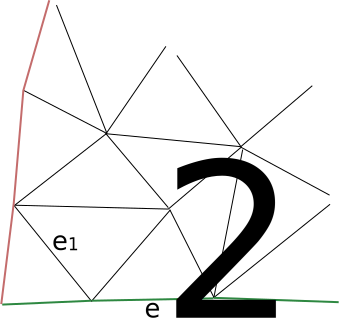
\includegraphics[width=\imagewidth]{contraction_arete_cas_1_1_avant}
	\label{fig:contraction_arete_cas_1_1_avant}
  }
  \hfill%
  \subbottom[Maillage résultant de la contraction de l'arête $e_2$.]{
	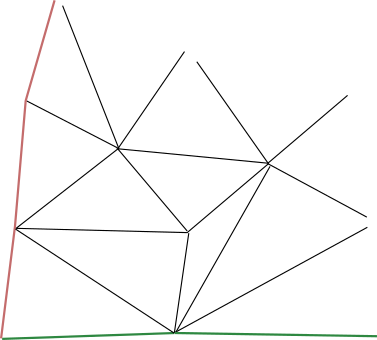
\includegraphics[width=\imagewidth]{contraction_arete_cas_1_1_apres}
	\label{fig:contraction_arete_cas_1_1_apres}
  }
  \hspace*{\fill}
  \caption{Deux cas possibles pour une arête dont les deux sommets ont un seul degré de liberté.}
  \label{fig:contraction_arete_cas_1_1}
  %
\end{figure}

Si $\ddl(p_1) < \ddl(p_2)$ on contracte $e$ vers le n\oe ud $p_1$. 
Si $\ddl(p_1) = \ddl(p_2)$ on contracte $e$ vers son milieu. Afin de localiser précisément ce milieu sur la surface \brep\ (\ie connaître l'entité \brep\ qui le supporte, ainsi que ses coordonnées paramétriques dans les carreaux de surface concernés), on calcule la projection sur la surface \brep\ du n\oe ud $p_1$ translaté d'un vecteur $\frac{p_2 - p_1}{2}$ (voir \autoref{fig:contraction_arete_milieu}), en suivant la procédure décrite dans la \autoref{section:projection_surface_composite}.

\setlength{\imagewidth}{50mm}
\begin{figure}
  \centering
  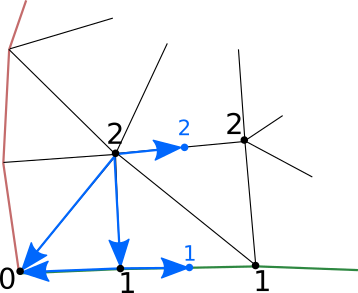
\includegraphics[width=\imagewidth]{contraction_arete_milieu}
  \caption{Placement du n\oe ud résultant de la contraction d'une arête. Le $\ddl$ de chaque n\oe ud concerné est indiqué à côté de celui-ci. Les flèches représentent les vecteurs déplacement à projeter pour chaque arête contractée.}
  \label{fig:contraction_arete_milieu}
\end{figure}


\subsubsection{Scission d'arête}
On insère un n\oe ud au milieu d'une arête. Comme pour la contraction d'arête, les coordonnées de ce milieu sont une nouvelle fois obtenue par la procédure de projection décrite dans la \autoref{section:projection_surface_composite}.
Cette fois, la projection du déplacement se fait en partant du sommet de l'arête ayant le plus grand nombre de degrés de liberté, comme illustré sur la \autoref{fig:scission_arete_milieu}.

\setlength{\imagewidth}{50mm}
\begin{figure}
  \centering
  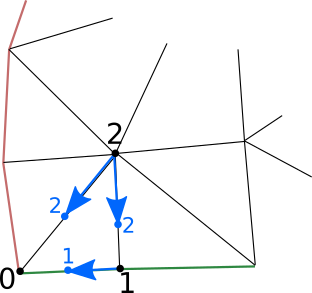
\includegraphics[width=\imagewidth]{scission_arete_milieu}
  \caption{Placement du nouveau n\oe ud résultant d'une scission d'arête. Le $\ddl$ de chaque n\oe ud concerné est indiqué à côté de celui-ci. Les flèches représentent les vecteurs déplacement à projeter pour chaque arête scindée.}
  \label{fig:scission_arete_milieu}
\end{figure}


\par\bigskip
\textit{
	[Bilan du chapitre et transition vers le chapitre suivant\ldots]
}
